Designovervejelser
Vi har valget at lave et program der planlægger skema for udskolingssektoren på en givende skole. Vi har valgt det skal være udskoling, altså 7, 8 og 9 klasse, for at kunne simulerede at lærerne kan have klasser på tværs af klassetrinene, og der ved vise at software løsningen kan løse problemet med sammenhængene forberedelsestimer for lærerne. Derudover skal programmet kunne planlægge skemaerne således at det er muligt at have samarbejde på tværs af parallel klasserne.  Da det er udskoling der arbejdes videre med, skal der specificeres hvilke parametre der gælder for disse klassetrin. Alle klassetrinene skal undervises i dansk, idræt, matematik, engelsk, historie, biologi, geografi, fysik og kemi, tysk eller fransk, derudover skal de have mulighed for at have et valgfag, det kunne f.eks. være fransk, billedkunst eller musik, alt efter hvad skolen har mulighed for at tilbyde. På syvende klassetrin er der også et praktisk fag som håndarbejde, sløjd eller hjemmekundskab på skemaet. De har til gengæld ikke kristendom på skemaet, da de har konfirmationsforberedelse\cite{lov2016}. Det fulde time antal for de forskellige fag kan ses på nedenstående skema:
\begin{figure}[!h]
  \centering
  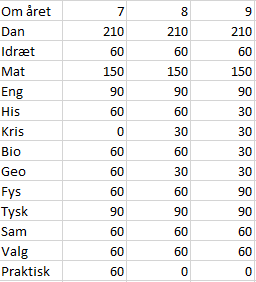
\includegraphics[width=\textwidth]{partials/graphics/antalaftimerpaaetaar.png}
  \caption{Tabel over timetallet for et år.}
  \label{fig:Timetalaar}
\end{figure}

Ugeligt vil det passe med følgende:
\begin{figure}[!h]
  \centering
  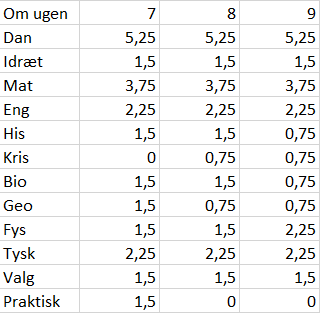
\includegraphics[width=\textwidth]{partials/graphics/antalaftimerpaaenuge.png}
  \caption{Tabel over timetallet for en uge.}
  \label{fig:Timetaluge}
\end{figure}

Derudover skal programmet opfylde de specifikke krav der bliver stillet af Sofiendahlskolen. Disse krav er at alle de tunge fag, som matematik dansk og fysik/kemi, skal lægges før elevernes middagspause, da eleverne som regl er mere ukoncentrerede efter middagspausen. Sofiendahlskolen vil også gerne have at lærerne har mere end en forberedelsestime adgangen. Lærerne mener at de ikke kan nå at forberede sig til de kommende lektioner på kun en time, derfor skal der helst være to eller flere forberedelsestimer ad gangen. På Sofiendahlskolen vægter de også samarbejde i mellem parallel klasser højt. Skemaet skal altså lægges således at visse fag forekommer på samme tidspunkt, så samarbejde mellem klasserne er muligt\cite{interview}. 

Det er også vigtigt at der ikke forekommer tomme lektioner inde midt på dagen.